
\documentclass{scrreprt}
%% verbatim -- > latex code listing
%% listing -- > matlab code listing
%% does not compile glossary or images at the moment
% \nonstopmode
\usepackage{morewrites}
\usepackage[
HomeHTMLFilename=index,     % Filename of the homepage.
%HTMLFilename={node-},       % Filename prefix of other pages.
IndexLanguage=english,      % Language for xindy index, glossary.
%latexmk,                    % Use latexmk to compile.
%   OSWindows,                  % Force Windows. (Usually automatic.)
mathjax,                    % Use MathJax to display math.
]{lwarp}
\usepackage{ifluatex}
\ifluatex\def\pdftexversion{140}\fi
\usepackage{import}
\title{ELEC 460 Course Notes}
\author{David Li}
\setcounter{tocdepth}{2} % Include subsections in the \TOC.
\setcounter{secnumdepth}{2} % Number down to subsections.
\setcounter{FileDepth}{0} % Split \HTML\ files at sections, in this case chapters?, 0 for chapters?
\booltrue{CombineHigherDepths} % Combine parts/chapters/sections
\setcounter{SideTOCDepth}{0} % Include subsections in the side\TOC
\HTMLAuthor{David Li} % Sets the HTML meta author tag.
\HTMLLanguage{en-US} % Sets the HTML meta language.
\HTMLDescription{Control Theory Notes}%

%\title{ELEC 460 Course Notes}
%\author{David Li}
\date{January 2018 --- April 2018}
\usepackage{tikz}
\usetikzlibrary{positioning}
\usetikzlibrary{shapes,arrows} 
\usepackage{float}

%\HTMLFirstPageTop{Name and \fbox{HOMEPAGE LOGO}}
%\HTMLPageTop{\fbox{LOGO}}
%\HTMLPageBottom{David Li,  \\ according the academic policy of \textbf{UVIC}, everything I do for a course is owned by me. Contact \url{lidavid@uvic.ca} for more info}
\CSSFilename{lwarp_sagebrush.css}


%% Trying out mdframed in lwarp
\usepackage[framemethod=tikz]{mdframed}
\newmdenv[
topline=false,
bottomline=false,
rightline=false,
innerrightmargin=0pt
]{siderule}
\newenvironment{note}%
{\begin{siderule}\textbf{Note:}}
	{\end{siderule}}

\usepackage{hyperref}

\hypersetup{colorlinks=true, linkcolor=blue, citecolor=black}
\usepackage{booktabs}
\usepackage{float}
\usepackage{multirow}
\usetikzlibrary{bending}
\usepackage{circuitikz}

%% https://tex.stackexchange.com/questions/301993/create-custom-note-environment-with-tcolorbox
\usepackage{enumitem}
\usepackage[listings,theorems]{tcolorbox}

%% See https://tex.stackexchange.com/questions/86711/tcolorbox-list-of-listings
% add tcblistings to \jobname.lol (list of listings), perhaps undefined in lwarp
%\makeatletter
%% add tcblistings to \jobname.lol (list of listings)
%\tcbset{
%	addtolol/.style={list entry={\kvtcb@title},add to list={lol}{section}},
%}
%\makeatother
\tcbuselibrary{listings}
\tcbuselibrary{breakable}
\newtcblisting[auto counter,number within=chapter]{matlaboutput}[2][]{sharp corners, breakable,
	fonttitle=\bfseries,colback=white, colframe=black!90, listing only, 
	listing options={language=Matlab, showstringspaces=false, breakatwhitespace=true, breaklines=true, tabsize=4}, 
	title=Matlab Output \thetcbcounter #1}

\newtcblisting[auto counter,number within=chapter]{pythonscript}[2][]{sharp corners, breakable,
	fonttitle=\bfseries, colback=gray!5, colframe=green!75, listing only, 
	listing options={language=python, showstringspaces=false, breakatwhitespace=true, breaklines=true, tabsize=4}, 
	title=Python Script \thetcbcounter  #1}

\newtcblisting[auto counter,number within=chapter]{latexcmd}[2][]{sharp corners, breakable,
	fonttitle=\bfseries,colback=gray!10, colframe=red!65, listing only, 
	listing options={language=TeX, showstringspaces=false, breakatwhitespace=true, breaklines=true, tabsize=4}, 
	title=Latex Commands \thetcbcounter  #1}

\newtcblisting[auto counter,number within=chapter]{bashcmd}[2][]{sharp corners, breakable,
	fonttitle=\bfseries,colback=gray!15, colframe=blue!65, listing only, 
	listing options={language=bash, showstringspaces=false, breakatwhitespace=true, breaklines=true, tabsize=4}, 
	title=Bash Script \thetcbcounter #1}
\definecolor{lightgray}{gray}{0.5}
% \definecolor{myText}{HTML}{2B2B2B}
\definecolor{fontColor}{HTML}{171717}
\setlength{\parindent}{0pt}

\makeindex

\usepackage{listings}
\definecolor{mygreen}{RGB}{28,172,0} % color values Red, Green, Blue
\definecolor{mylilas}{RGB}{170,55,241}
\lstset{language=Matlab,%
	%basicstyle=\color{red},
	breaklines=true,%
	morekeywords={matlab2tikz},
	keywordstyle=\color{blue},%
	morekeywords=[2]{1}, keywordstyle=[2]{\color{black}},
	identifierstyle=\color{black},%
	stringstyle=\color{mylilas},
	commentstyle=\color{mygreen},%
	showstringspaces=false,%without this there will be a symbol in the places where there is a space
	%numbers=left,%
	%numberstyle={\tiny \color{black}},% size of the numbers
	%numbersep=9pt, % this defines how far the numbers are from the text
	emph=[1]{for,end,break},emphstyle=[1]\color{red}, %some words to emphasise
	%emph=[2]{word1,word2}, emphstyle=[2]{style},  
	%captionpos=b,
	%caption={Matlab Code Snippet:},
}

\usepackage{amsthm,amsmath,amssymb}
\usepackage{listings}
\theoremstyle{plain}
\newtheorem{theorem}{Theorem}[section]
\newtheorem{corollary}{Corollary}[theorem]
%\newtheorem{corollary}{Corollary}[section]
\newtheorem{lemma}{Lemma}[theorem]
%\newtheorem{example}{Example}[theorem]


\theoremstyle{definition}
\newtheorem{definition}{Definition}[section]
\newtheorem{example}{Example}[section]
\theoremstyle{remark}
\newtheorem*{remark}{Remark}

%\theoremstyle{proof}
%\newtheorem{myproof}{Proof}[section]
\renewcommand\qedsymbol{$\blacksquare$}
%\newtheorem{definition}{Definition}[section]
%% Added for bibilography and title page
% Using pandoc approach, convert to html and copy and paste back in
\usepackage[backend=bibtex,sorting=none]{biblatex}	% Sort by citation order
\addbibresource{../textbooks.bib}		% Load bibliography

\usepackage{marginnote}

\usepackage{algorithmicx}

%%% New package that I didn't know worked with lwarp
%\usepackage{changebar}
%\setlength{\changebarsep}{2ex}
\usepackage[xindy]{glossaries}
%\setglossarystyle{mcolalttree}
\newglossaryentry{Actuator}
{
	name = {Actuator},
	description = {
		 In a \gls{closedLoop} control system, that part of the final control element that translates the controller output into an action by the control device.}
}

\newglossaryentry{conSys}
{
	name = {Control System},
	description = {
		A control system is an interconnection of components forming a system configuration that will provide a desired system response.
	}
}
\newglossaryentry{openLoop}
{
	name = {open-loop control system},
	description = {
		An open-loop control system utilizes an actuating device to control the process
		directly without using feedback.
	}
}
\newglossaryentry{closedLoop}{
	name={closed-loop control system},
	description={A closed-loop control system uses a measurement of the output and feedback of this signal to compare it with the desired output (reference or command).
	}
}

\newglossaryentry{SISO}
{
	name = {Single Input Single Output},
	description = {
		In control engineering, a single-input and single-output (SISO) system is a simple single variable control system with one input and one output. SISO systems are typically less complex than multiple-input multiple-output (MIMO) systems. Frequency domain techniques for analysis and controller design dominate SISO control system theory. }
}

\newglossaryentry{MIMO}
{
	name = {Multiple Input Multiple Output},
	description = {
		In control engineering, systems with more than one input and/or more than one output are known as Multi-Input Multi-Output systems, or they are frequently known by the abbreviation MIMO. MIMO systems that are lumped and linear can be described easily with state-space equations.}
}
\newglossaryentry{LTI}
{
	name = {linear time-invariant},
	description = {
		\textbf{Linear time-invariant systems} (LTI systems) are a class of systems used in signals and systems that are both linear and time-invariant. Linear systems are systems whose outputs for a linear combination of inputs are the same as a linear combination of individual responses to those inputs. Time-invariant systems are systems where the output does not depend on when an input was applied. 
	}
}

\newglossaryentry{cornFreq}
{
	name = {Corner Frequency},
	description = {
	 For first order systems, the corner frequency is the frequency where the magnitude starts to roll-off (3dB below the steady-state gain) and the phase shift is -45 degrees. Also: corner frequency = 1/(time constant) rads/s.
	}
}

\newglossaryentry{controlGain}
{
	name = {Controller Gain},
	description = {
		This is another term for the "P" part of the PID controller. The more gain a controller has the faster and potentially more oscillatory the loop response will be.
	}
}

\newglossaryentry{critDamp}
{
	name = {critically-damped},
	description = {
		A linear system that has the fastest response without any overshoot is said to be critically damped.
	}
}

\newglossaryentry{bodeDia}
{
	name = {bode diagram},
	description = {
		Graphical display of the frequency response with magnitude and phase both plotted against frequency on the horizontal axis.
	}
}

%%%%%%%%%%%%%%%%%%%%%%%%%%%%%%%%%%%%%%%%%%%%%%%%%%%%%%%%%%%%%%%%%%%
%%%%	Command to ensure  glossary can be properly updated/printed %%%%%%%%%%
%%%% makeindex -l -s ELEC360Notes.ist -o ELEC360Notes.gls ELEC360Notes.glo %%%%%%%%%
%%%%	Use name of latex document								%%%%%%%%%%%
%%%%%%%%%%%%%%%%%%%%%%%%%%%%%%%%%%%%%%%%%%%%%%%%%%%%%%%%%%%%%%%%%%%%%%
\makeglossaries

\usepackage{moreverb}
\usepackage{epigraph}
\usepackage{csquotes}
\usepackage{makeidx}\makeindex
\usepackage{pgfplots}
\usepackage{steinmetz}
\begin{document}
%% Print Title Page
\makeatletter
% Create \printauthor command which will display contact info                     
\def\printauthor{%                  
	{\large \@author}}              
\makeatother
% Honestly, if footcite works that would be adequate for me
\author{%
	\textbf{Name: }  David Li \\
	\textbf{Student Number:} V00818631	\\
	\textbf{Term}  3A  \\
	\textit{Discipline:} Computer Engineering \\  \vspace{4pt}
	\textit{Email:} \href{mailto:lidavid@uvic.ca}{lidavid@uvic.ca}
}

\maketitle
	
\begin{titlepage}
	%\AddToShipoutPicture*{\BackgroundPic}
	\begin{center}
		%		{\vspace*{3pt} }
		{\Huge \textsc{Faculty of Electrical and Computer Engineering} \\ \vspace{4pt}}
		{\Huge \textsc{Control Theory II } \\ \vspace{4pt}}  
		\rule[13pt]{1\textwidth}{1pt} \\ \vspace{1pt}
		{\LARGE \textbf{{\textsc{Digital Control Systems}}} \\ Spring 2018 --- \textit{Dr. Pan Agathoklis} \\ }
		{\Large \textsc{Required Text: Discrete Time Control Systems} \\} 
		\vspace{4pt} 
		{\Large \textsc{Spring 2018}} \\ 
		\vspace{20pt}
		{\Large \textsc{Victoria, British Columbia, Canada} \\ \vspace{45pt} }
		
		\begin{minipage}{0.96\linewidth}
			\begin{flushright}
				{
					\large \textit{Course Website} \href{http://www.ece.uvic.ca/~panagath/ELEC460/ELEC460.html}{ELEC 460}  \\
					\textsc{\textbf{Course Assessment:}} \\
					Assignments	: 5 \% \\
					Mid-term	: 35 \% Monday, February 5, 2018 \\
					Final	: 60 \%} \\
			\end{flushright}
%		\begin{minipage}{0.02\linewidth}
%			\rule[0pt]{1pt}{110pt} 
%		\end{minipage}
		\end{minipage}

%		\\ \vspace{10pt}
		{\Large \textsc{\today} \\ \vspace{15pt}
			{\Large \textsc{In partial fulfillment of the academic requirements of this course. \\
				}
			}	
		}
		
	\end{center}
\end{titlepage}
\tableofcontents
\listoffigures
\listoftables
\lstlistoflistings

\addcontentsline{toc}{chapter}{Index}
\printindex

\part{Control Theory}
\chapter{Course Information}
\begin{quote}
\textbf{Course Objectives:} Introduction in the analysis and design of digital and/or analog control systems.
Understanding the mathematical tools used in control system analysis and design.
Design digital controllers for systems in input-output description and/or state-space description.

\textbf{Syllabus ELEC 460:} Sampling in Control Systems. The z-transform and response between sampling instants. Analysis of
sampled data systems and stability testing. State-space analysis and design of continuous and discrete systems.
Controllability, observability and zero input stability analysis. Pole placement techniques. (Prerequisite: 360)

\end{quote}

\textbf{Description}
\begin{itemize}
\item[---] Apply z-Transform to solve difference
\item[---] Discuss description of discrete systems using transfer functions and state-space description
\item[---] Analyse stability, transient and steady state system response
\item[---] Demonstrate the digital implementation of lead and lag compensators
\item[---] Analyse controllability and observability for systems in state space description
\item[---] Design linear state feedback controllers using pole-placement
\item[---] Apply state observers for state estimation of linear systems in state-space description
\end{itemize}

\textbf{Assessment:}
\begin{table}
\begin{tabular}{c c }
Assignments: & 5 \% \\
Mid-term 35 \% & Date: Monday, February 5, 2018 \\
Final &  60 \% 
\end{tabular}
\caption{Course Assessment}
\end{table}

\begin{description}
	\item[Phase Margin] (PM) --- $\phi_m$, the difference from the phase plot and 180 degrees at the gain cut-off point.
	\item[Gain Margin] (GM) ---  at the  frequency cut-off point, the difference from the magnitude plot and 0 is the GM, $K$.
	\item[Bode Plot] --- frequency domain plot that contains $\phi_m$, and $K$, see \gls{bodeDia}.
	\item[Root Locus] --- Used in assignment 1, to help determine the damping ratio.
\end{description}
\chapter{Introduction and Review}
For this course, %\hyperlink{ref-MatlabCST}{Matlab Control Systems} 
\cite{MatlabCST} and \cite{MatlabSMT} will be used extensively.


%For instance I can use the same \footnote{\hyperlink{ref-textbook:kuo}{Kuo Textbook}} more \footnote{\hyperlink{ref-book:129711}{Some Textbook}} than  \footnote{\hyperlink{ref-MatlabCST}{Control System Toolbox}}
% once.

\footnotetext{footnote with two references}
\begin{figure}
\begin{lateximage}
	\tikzstyle{block} = [draw, fill=blue!20, rectangle, minimum height=3em, minimum width=4em]
	\tikzstyle{controller} = [draw, fill=green!20, rectangle, minimum height=3em, minimum width=4em]
	\tikzstyle{sum} = [draw, fill=blue!20, circle, node distance=1cm]
	\tikzstyle{input} = [coordinate]
	\tikzstyle{output} = [coordinate]
	\begin{tikzpicture}[auto]
	% Nodes
	\node [input] (input) {};
	\node [sum, right = 1cm of input] (sum) {};
	\node [controller, right = 1cm of sum] (con1) {A/D};
	\node [controller, right = 1cm of con1] (con2) {Control};
	\node [controller, right = 1cm of con2] (system2) {D/A};
	\node [block, right = 1cm of system2] (system3) {Process};
	\node [output, right = 2cm of system3] (output) {};
	\node [input, below = 0.5cm of con2] (m) {};
	% Arrows
	\draw [draw,->] (input) -- node {$Z_{real}$} (sum);
	\draw [->] (sum) -- (con1);
	\draw [->] (con1) -- (con2);
	\draw [->] (con2) -- node {$$} (system2);
	\draw [->] (system2) -- node {$$} (system3);
	\draw [->] (system3) -- node (y) {$Z$}(output);
	\draw [-] (y) |- (m) {} ;
	\draw [->] (m) -| node[pos=0.99] {$-$}  node [near end] {} (sum);
	\draw[thick,dotted]     ($(con1.north west)+(-0.5,0.15)$) rectangle ($(system2.south east)+(0.5,-0.15)$);
	\node [above = 0.25cm of con2] {Digital Controller};
	%\node [above = of near end] {+};
	\end{tikzpicture}
\end{lateximage}
\end{figure}


\paragraph{Z Transforms}
\begin{center}
\large
\begin{tabular}{|c|c|}
\hline
\multicolumn{2}{|c|}{\textbf Table of Z Transforms}\\
\hline
$(x_k)_{k=0}^\infty$&  $Z \left[(x_k)_{k=0}^\infty \right]$\\
\hline
&\\
$x_k =\delta_k= \left\{ \begin{array}{ll} 1 & k = 0\\
   				 0 & k > 0
		\end{array} \right.$             & 1\\
(unit pulse)                 & \\
$x_k = r^k$ & $\frac{z}{z-r}$\\

$x_k = kr^{k-1}$ & $\frac{z}{(z-r)^2}$\\

\hline
\end{tabular}
\end{center}
{\textbf First shift theorem} (delaying):  if ${{Z}}[(x_k)]=X(z)$then
\[
{{Z}}[(x_{k-k_0})]=\frac{1}{z^{k_0}}X(z)
\]
where $x_k=0$for $k<0$.

\noindent {\textbf Second shift theorem} (advancing): if ${Z}[(x_k)]=X(z)$then
\[
{Z}[(x_{k+1})]=zX(z)-zx_0
\]
and
\[
{Z}[(x_{k+2})]=z^2X(z)-z^2x_0-zx_1
\]


\begin{table}[h]
	\begin{center}
	\begin{tabular}{c|c|c|c}
		\toprule 
		QUANTITY & SYMBOL & UNIT & UNIT ABBERVIATION 	\\
		Time & t & second & s				\\
		Frequency (cyclic) & f & hertz & Hz \\
		Frequency (radian) & $\omega $& radian/sec & rad/s	\\
		Phase angle &$\theta $, $\varphi $ & degree or radian & $^{\circ}$ or rad \\
		Energy & w & joule & J 	\\
		Power & p & watt & W	\\
		Charge & q  &coulomb & C	\\
		Current & i & ampere  &A	\\
		Electric field & E & volt/meter& V/m	\\
		Voltage & v & volt &V	\\
		Impedence & Z & ohm & $\varOmega$	\\
		Admittance &Y &siemen &S	\\
		Resistance &R &ohm &$\varOmega$	\\
		Conductance& G &siemen &S	\\
		Reactance &X &ohm &$\varOmega$	\\
		Susceptance &B &siemen& S	\\
		Inductance, self &L &henry& H	\\
		Inductance, mutual& M &henry& H	\\
		Capacitance& C& farad &F	\\
		Magnetic flux& $\phi$& weber &wb	\\
		Flux linkages& $\lambda$& weber-turns& wb-t	\\
		Power ratio& $log_{10}\frac{p_2}{p_1}$& Bel &B	\\
		\bottomrule
	\end{tabular}
	\caption{Electric Quantities}
\end{center}
\end{table}

 \begin{table}[h]
	
	\begin{center}
			\begin{tabular}{cccccc}
				\toprule 
				\multirow{1}{*}{}	& \multicolumn{2}{c}{\multirow{ 2}{*}{I-V RELATIONSHIPS}} &	\multicolumn{3}{c}{IMPENDENCE}  \\ \cline{4-6}
				& &	&  PHASOR-DOMAIN & s-DOMAIN & \\ \hline
				Resistor	& $v_R(t)=i_R(t) \times R=\dfrac{i_R(t)}{G}$& $i_R(t)=\dfrac{v_R(t)}{R}=v_R(t) \times G$& $ Z_R $ & R & R\\ \hline
				Inductor	& $v_L(t)=L\times \dfrac{ \partial i_L(t)}{\partial t} $& $i_L(t)=\dfrac{1}{L} \int_{0}^{t} v_L(x)dx+ i_L(0)$& $ Z_L $ &$ j\omega L$ & Ls\\ \hline
				Capacitor	& $v_C(t)=dfrac{1}{C}\int_{0}^{t} i_C(x)dx+ v_C(0)$& $i_C(t)=C\times \dfrac{\partial v_C(t)}{\partial t} $& $ Z_C $ & $ \dfrac{1}{j\omega C} $& $\dfrac{1}{Cs}$\\ 
				\bottomrule
			\end{tabular}
		\caption{Basic Circuit Relations}
	\end{center}
\end{table}


where 

\noindent{\textbf First shift theorem:} If $L(f(t))=F(s)$ then
$$ {\mathcal L}\left(e^{at}f(t)\right)=F(s-a).$$
{\textbf Third shift theorem:} If ${L}(f(t))=F(s)$ then
$$ {\mathcal L}\left(H_a(t)f(t-a)\right)=e^{-as}F(s).$$
\chapter{Other Useful Concepts}

\section{Steady-state error}

\subsection{Definition}

Consider a feedback system as in Fig.~ \ref{fig:sse}.

%% Consider adding ELEC460Notes-figure0.png, .. ELEC460Notes-figuren.png by using an if, else statement so I can get native html output using pandoc.
\begin{figure}
		\centering
\begin{lateximage}
	\tikzstyle{block} = [draw, fill=blue!20, rectangle, minimum height=3em, minimum width=4em]
	\tikzstyle{block2} = [draw, fill=blue!20, rectangle, minimum height=2em, minimum width=2em]
	\tikzstyle{sum} = [draw, fill=blue!20, circle, node distance=1cm]
	\tikzstyle{input} = [coordinate]
	\tikzstyle{output} = [coordinate]
	\begin{tikzpicture}[auto, >=latex']
	% Nodes
	\node [input] (input) {};
	\node [sum, right = 1cm of input] (sum) {};
	%\node [block2, right = 1cm of sum] (system) {$K$};
	\node [block, right = 1cm of sum] (system2) {$G$};
	\node [output, right = 2cm of system2] (output) {};
	\node [block, below = 0.5cm of system2] (h) {$H$};
	% Arrows
	\draw [draw,->] (input) -- node {$R$} (sum);
	\draw [->] (sum) -- node {$E$} (system2);
	%\draw [->] (system) -- (system2);
	\draw [->] (system2) -- node (y) {$C$}(output);
	\draw [-] (y) |- (h) {} ;
	\draw [->] (h) -| node[pos=0.99] {$-$}  node [near end] {} (sum);
	\end{tikzpicture}  
\end{lateximage}
	\caption{Error signal: $E=R-C$}
\label{fig:sse}
\end{figure}
The steady-state error (if it exists) is defined by
\begin{align*}
	e_{ss} := \lim_{t\to\infty} e(t).
\end{align*}

If the system is stable, one can apply the Finaly Value Theorem to obtain
\[
\lim_{t\to\infty} e(t) = \lim_{s\to 0} sE(s).
\]
In general, one would like the steady-state error to be as small as
possible, ideally zero.

\subsection{System type and steady-state error}

 \marginnote{This is a margin note using the geometry package, set at 3cm vertical offset to the line it is typeseted.}[3cm]
In general, to calculate the steady-state error, one uses the FVT as
in equation~ %(\ref{eq:sse}).

\reversemarginpar
\marginnote{This is a margin note using the geometry package, set at 5cm 
	vertical offset to the first line it is typeset.}[3cm]

 However, if the system is stable and
\emph{unity-feedback}, then one can determine the system type and use
this information to obtain the steady-state error much more easily. 
\reversemarginpar
\marginnote{This is a margin note using the geometry package, set at 5cm 
	vertical offset to the first line it is typeset.}[3cm]
Let $G$ be the feedforward transfer function. Assume that $G$ is
written as
\[
G=\frac{N(s)}{s^kD(s)},
\]
where $N$ and $D$ are not factorizable by $s$. Then the type of the
system is given by the integer $k$. Fig.~\ref{fig:systype} shows the
general form of systems of types 1, 2 and 3.

\begin{figure}
\begin{lateximage}

	\hspace{1.5cm}\textbf{Type 0}\hspace{3cm}\textbf{Type
		1}\hspace{3cm}\textbf{Type 2}\\
	\vspace{0.1cm} 
	
	\centering \tikzstyle{block} = [draw, fill=blue!20,
	rectangle, minimum height=3em, minimum width=3em]
	\tikzstyle{controller} = [draw, fill=red!20, rectangle, minimum
	height=3em, minimum width=4em] \tikzstyle{sum} = [draw,
	fill=blue!20, circle, node distance=1cm] \tikzstyle{input} =
	[coordinate] \tikzstyle{output} = [coordinate]
	\begin{tikzpicture}[auto, >=latex']
	% Nodes
	\node [input] (input) {};
	\node [sum, right = 0.5cm of input] (sum) {};
	\node [block, right = 0.5cm of sum] (system) {$\frac{N_0(s)}{D_0(s)}$};
	\node [output, right = 1cm of system] (output) {};
	\node [input, below = 0.5cm of system] (m) {};
	% Arrows
	\draw [draw,->] (input) -- node {$R$} (sum);
	\draw [->] (sum) -- node {} (system);
	\draw [->] (system) -- node (y) {$C$}(output);
	\draw [-] (y) |- (m) {} ;
	\draw [->] (m) -| node[pos=0.99] {$-$}  node [near end] {} (sum);
	\end{tikzpicture}  
	\hspace{0.5cm}
	\begin{tikzpicture}[auto, >=latex']
	% Nodes
	\node [input] (input) {};
	\node [sum, right = 0.5cm of input] (sum) {};
	\node [block, right = 0.5cm of sum] (system) {$\frac{N_1(s)}{sD_1(s)}$};
	\node [output, right = 1cm of system] (output) {};
	\node [input, below = 0.5cm of system] (m) {};
	% Arrows
	\draw [draw,->] (input) -- node {$R$} (sum);
	\draw [->] (sum) -- node {} (system);
	\draw [->] (system) -- node (y) {$C$}(output);
	\draw [-] (y) |- (m) {} ;
	\draw [->] (m) -| node[pos=0.99] {$-$}  node [near end] {} (sum);
	\end{tikzpicture}  
	\hspace{0.5cm}
	\begin{tikzpicture}[auto, >=latex']
	% Nodes
	\node [input] (input) {};
	\node [sum, right = 0.5cm of input] (sum) {};
	\node [block, right = 0.5cm of sum] (system) {$\frac{N_2(s)}{s^2D_2(s)}$};
	\node [output, right = 1cm of system] (output) {};
	\node [input, below = 0.5cm of system] (m) {};
	% Arrows
	\draw [draw,->] (input) -- node {$R$} (sum);
	\draw [->] (sum) -- node {} (system);
	\draw [->] (system) -- node (y) {$C$}(output);
	\draw [-] (y) |- (m) {} ;
	\draw [->] (m) -| node[pos=0.99] {$-$}  node [near end] {} (sum);
	\end{tikzpicture}  
\end{lateximage}
	\caption{Systems of types 0, 1 and 2. Note that $N_0, N_1, N_2, D_0,
	D_1, D_2$ should not be factorizable by $s$.}
\label{fig:systype}
\end{figure}
Let us carry further the computation of the steady-state error for a
stable unity-feedback system.
\[
sE(s) = s(R(s)-C(s)) = s\left(R(s)-\frac{G(s)}{1+G(s)}R(s)\right)=\frac{s}{1+G(s)}R(s).
\]

For unit-step input, one has $R(s)=1/s$. Thus,
\[
sE(s) = \frac{s}{1+G(s)}*\frac{1}{s} = \frac{1}{1+G(s)}
\xrightarrow[s\to 0]{}\frac{1}{1+\lim_{s\to 0}G(s)}.
\]
For a system of type 0, one has
\[
\lim_{s\to 0}G(s) = \lim_{s\to 0}\frac{N_0(s)}{D_0(s)} = \frac{N_0(0)}{D_0(0)}.
\]
Thus, the steady-state error of a system of type 0 for unit-step input
is given by
\[
e_{ss} = \frac{1}{1+\frac{N_0(0)}{D_0(0)}}.
\]

Carrying out similar calculations, one obtains the following table,
which shows the steady-state errors of systems of types 0, 1, 2, 3 for
unit-step, unit-ramp and unit-parabola inputs.

\begin{table}[htp]
	\centering
	\begin{tabular}{|c|c|c|c|}
		\hline
		System type&Step input&Ramp input&Parabolic input\\\hline
		Type 0&$\frac{1}{1+K_p}$&$\infty$&$\infty$\\\hline
		Type 1&0&$\frac{1}{K_v}$&$\infty$\\\hline
		Type 2&0&0&$\frac{1}{K_a}$\\\hline
		Type 3&0&0&0 \\ \hline
	\end{tabular}
	\caption{Steady-state errors of systems of different types and for
		different inputs.}
	\label{tab:systype}
\end{table}

The constants $K_p$, $K_v$, and $K_a$ are defined as below
\begin{itemize}
	\item for a system of type 0, $K_p:=\frac{N_0(0)}{D_0(0)}$ (position constant);
	\item for a system of type 1, $K_v:=\frac{N_1(0)}{D_1(0)}$ (velocity constant);
	\item for a system of type 2, $K_a:=\frac{N_2(0)}{D_2(0)}$
	(acceleration constant).
\end{itemize}

\subsection{Other Block Diagrams}
In the Laplace domain, we have
\[
I = K_D(sZ_{real}-sZ) + K_P(Z_{real}-Z) = (K_Ds+K_P)(Z_{real}-Z),
\]
which leads to the following block diagram.

\begin{figure}
\begin{lateximage}

	\label{fig:examplesystempd}
	\centering
	\tikzstyle{block} = [draw, fill=blue!20, rectangle, minimum height=3em, minimum width=4em]
	\tikzstyle{controller} = [draw, fill=red!20, rectangle, minimum height=3em, minimum width=4em]
	\tikzstyle{sum} = [draw, fill=blue!20, circle, node distance=1cm]
	\tikzstyle{input} = [coordinate]
	\tikzstyle{output} = [coordinate]
	\begin{tikzpicture}[auto, >=latex']
	% Nodes
	\node [input] (input) {};
	\node [sum, right = 1cm of input] (sum) {};
	\node [controller, right = 1cm of sum] (system) {$K_D s + K_P$};
	\node [block, right = 1cm of system] (system2) {$\frac{k}{ms^2}$};
	\node [output, right = 2cm of system2] (output) {};
	\node [input, below = 0.5cm of system] (m) {};
	% Arrows
	\draw [draw,->] (input) -- node {$Z_{real}$} (sum);
	\draw [->] (sum) -- node {} (system);
	\draw [->] (system) -- node {$I$} (system2);
	\draw [->] (system2) -- node (y) {$Z$}(output);
	\draw [-] (y) |- (m) {} ;
	\draw [->] (m) -| node[pos=0.99] {$-$}  node [near end] {} (sum);
	\end{tikzpicture}  
\end{lateximage}
	\caption{Proportional-derivative control.}
\end{figure}
\begin{figure}
	\label{fig:lag}
	\centering
\begin{lateximage}

	\tikzstyle{block} = [draw, fill=blue!20, rectangle, minimum height=3em, minimum width=4em]
	\tikzstyle{controller} = [draw, fill=red!20, rectangle, minimum height=3em, minimum width=4em]
	\tikzstyle{sum} = [draw, fill=blue!20, circle, node distance=1cm]
	\tikzstyle{input} = [coordinate]
	\tikzstyle{output} = [coordinate]
	\begin{tikzpicture}[auto, >=latex']
	% Nodes
	\node [input] (input) {};
	\node [sum, right = 1cm of input] (sum) {};
	\node [controller, right = 1cm of sum] (con1) {$\frac{s+p_c}{s+z_c}$};
	\node [controller, right = 1cm of con1] (con2) {$K_D s + K_P$};
	\node [block, right = 1cm of con2] (system2) {$\frac{k}{ms^2}$};
	\node [output, right = 2cm of system2] (output) {};
	\node [input, below = 0.5cm of con2] (m) {};
	% Arrows
	\draw [draw,->] (input) -- node {$Z_{real}$} (sum);
	\draw [->] (sum) -- (con1);
	\draw [->] (con1) -- (con2);
	\draw [->] (con2) -- node {$I$} (system2);
	\draw [->] (system2) -- node (y) {$Z$}(output);
	\draw [-] (y) |- (m) {} ;
	\draw [->] (m) -| node[pos=0.99] {$-$}  node [near end] {} (sum);
	\end{tikzpicture}  

\end{lateximage}
	\caption{Lag compensation in series with PD control.}
\end{figure}

\begin{figure}
	\label{fig:integral}
\begin{lateximage}

	\centering
	\tikzstyle{block} = [draw, fill=blue!20, rectangle, minimum height=3em, minimum width=4em]
	\tikzstyle{controller} = [draw, fill=red!20, rectangle, minimum height=3em, minimum width=4em]
	\tikzstyle{sum} = [draw, fill=blue!20, circle, node distance=1cm]
	\tikzstyle{input} = [coordinate]
	\tikzstyle{output} = [coordinate]
	\begin{tikzpicture}[auto, >=latex']
	% Nodes
	\node [input] (input) {};
	\node [sum, right = 1cm of input] (sum) {};
	\node [controller, right = 1cm of sum] (system) {$\frac{K}{s}$};
	\node [block, right = 1cm of system] (system2) {$\frac{1}{Ts+1}$};
	\node [output, right = 2cm of system2] (output) {};
	\node [input, below = 0.5cm of system] (m) {};
	% Arrows
	\draw [draw,->] (input) -- node {$R$} (sum);
	\draw [->] (sum) -- node {} (system);
	\draw [->] (system) --  (system2);
	\draw [->] (system2) -- node (y) {$C$}(output);
	\draw [-] (y) |- (m) {} ;
	\draw [->] (m) -| node[pos=0.99] {$-$}  node [near end] {} (sum);
	\end{tikzpicture}  

\end{lateximage}
	\caption{First order system with integral controller.}
\end{figure}
	
\chapter{Example commands}

\section{Testing out matlab}
\begin{matlaboutput}{}
	% M-file: prob7_17.m
	% M-file create a plot of the induced torque power
	% converted power out and efficiency of the induction
	% motor of Problem 7-14 as a function of slip.
	% First, initialize the values needed in this program.
	r1 = 0.075; % Stator resistance
	x1 = 0.170; % Stator reactance
	r2 = 0.065; % Rotor resistance
	x2 = 0.170; % Rotor reactance
	xm = 7.2; % Magnetization branch reactance
	v_phase = 440 / sqrt(3); % Phase voltage
	n_sync = 3000; % Synchronous speed (r/min)
	w_sync = 314.2; % Synchronous speed (rad/s)
	p_mech = 1000; % Mechanical losses (W)
	p_core = 1100; % Core losses (W)
	p_misc = 150; % Miscellaneous losses (W)
	% Calculate the Thevenin voltage and impedance from Equations
	% 7-41a and 7-43.
	v_th = v_phase * ( xm / sqrt(r1^2 + (x1 + xm)^2) );
	z_th = ((j*xm) * (r1 + j*x1)) / (r1 + j*(x1 + xm));
	r_th = real(z_th);
	x_th = imag(z_th);
\end{matlaboutput}

\section{Testing out Python}
\begin{pythonscript}{}
# -*- coding: utf-8 -*-
"""
Created on Sun Dec 31 09:50:49 2017

@author: David Li
Helper script to create lwarpnotes, latex file should be set to \nonstopmode
"""

import subprocess,os,sys
# consider using command line arguments to prompt the user for input if being run from command line or hardcoded value if any arguements are passed through.
if len(sys.argv) > 1:
input_tex_file = 'ELEC460Notes.tex'
else:
input_tex_file = input("Enter the tex name. ")
input_name, input_extension = os.path.splitext(input_tex_file)
if os.path.isfile(input_tex_file):
print('Proceeding to produce: ' + input_name + '.pdf and ' + input_name +'_html' + '\n' )
else:
\end{pythonscript}

\section{Testing out Bash}
Hmm, cannot do this
\begin{bashcmd}{}
	
pdflatex file
pdflatex file_html.tex
lwarpmk limages
lwarpmk html
lwarpmk pdftohtml
\end{bashcmd}

% Do not nest tags such as lstlisting and example
\begin{example}
	Testing out the examples
\end{example}

\section{Testing out Latex}
\begin{latexcmd}{}
	Testing out latex commands
	Tiks
\end{latexcmd}

This is some garbo text,

\section{Testing out Bash}


\begin{bashcmd}{}
	Testing out latex commands
	Tiks
\end{bashcmd}

\begin{lemma}
	A lemma to go with my Theorem!
\end{lemma}
%------------------------------------------------
Shocked that this still doesn't work hmm


\begin{theorem}{\textbf{Circuits}}
	A set $\mathcal{D}(G)$ in dense in $L^2(G)$, $|\cdot|_0$. 
\end{theorem}
\section{Example Definitions}\index{Definitions}

% Hmm check script again
\begin{lstlisting}[caption={This is a caption}]
hmm
\end{lstlisting}
This is an example of a definition. A definition could be mathematical or it could define a concept.
\begin{lstlisting}[caption={This is a caption}]
foo bar = 5;
\end{lstlisting}


\begin{verbatim}
	\tikzstyle{block} = [draw, fill=blue!20, rectangle, minimum height=3em, minimum width=4em]
\tikzstyle{block2} = [draw, fill=blue!20, rectangle, minimum height=2em, minimum width=2em]
\tikzstyle{sum} = [draw, fill=blue!20, circle, node distance=1cm]
\tikzstyle{input} = [coordinate]
\tikzstyle{output} = [coordinate]
\begin{tikzpicture}[auto, >=latex']
% Nodes
\node [input] (input) {};
\node [sum, right = 1cm of input] (sum) {};
%\node [block2, right = 1cm of sum] (system) {$K$};
\node [block, right = 1cm of sum] (system2) {$G$};
\node [output, right = 2cm of system2] (output) {};
\node [block, below = 0.5cm of system2] (h) {$H$};
% Arrows
\draw [draw,->] (input) -- node {$R$} (sum);
\draw [->] (sum) -- node {$E$} (system2);
%\draw [->] (system) -- (system2);
\draw [->] (system2) -- node (y) {$C$}(output);
\draw [-] (y) |- (h) {} ;
\draw [->] (h) -| node[pos=0.99] {$-$}  node [near end] {} (sum);
\end{tikzpicture} 
\end{verbatim}


%\begin{verbatim*}
%Text enclosed inside \texttt{verbatim} environment 
%is printed directly 
%and all \LaTeX{} commands are ignored.
%\end{verbatim*}
%
%\begin{verse}
%	A verse starts here,
%	A hero rises,
%	The end he is dead.
%\end{verse}
\begin{quote}
	Legends will fall
\end{quote}

\hyphenquote{UKenglish}{quote with UK English hyphenation}

\epigraph{I recall seeing a package to make quotes}{Snowball}

\begin{verse}
	
Because of limitations in how pandoc works, I suppose I could mix and max using bash and * to load all the individual files, in fact maybe that's what I'll do, take a month worth of notes and check the loading times and if it's not to bad I'll continue writing notes on my computer, but if I do it like that then I will have to either bring my computer to class or write them down by hand. Seems that using texstudio to compile lwarp is a mistake stick to perl command line.

\end{verse}

\begin{definition}
	Given a vector space $E$, a norm on $E$ is an application, denoted $||\cdot||$, $E$ in $\mathbb{R}^+=[0,+\infty[$ such that:
	\begin{align}
	& ||\mathbf{x}||=0\ \Rightarrow\ \mathbf{x}=\mathbf{0}\\
	& ||\lambda \mathbf{x}||=|\lambda|\cdot ||\mathbf{x}||\\
	& ||\mathbf{x}+\mathbf{y}||\leq ||\mathbf{x}||+||\mathbf{y}||
	\end{align}
\end{definition}

%------------------------------------------------

\section{Notations}\index{Notations}

\begin{example}
	Given an open subset $G$ of $\mathbb{R}^n$, the set of functions $\varphi$ are:
	\begin{enumerate}
		\item Bounded support $G$;
		\item Infinitely differentiable;
	\end{enumerate}
	a vector space is denoted by $\mathcal{D}(G)$. 
\end{example}

%------------------------------------------------

\section{Remarks}\index{Remarks}

This is an example of a remark.

\begin{remark}
	The concepts presented here are now in conventional employment in mathematics. Vector spaces are taken over the field $\mathbb{K}=\mathbb{R}$, however, established properties are easily extended to $\mathbb{K}=\mathbb{C}$.
\end{remark}

\begin{theorem}
	Testing out the theorems
\end{theorem}
%------------------------------------------------

\section{Corollaries}\index{Corollaries}

This is an example of a corollary.

\begin{corollary}
	The concepts presented here are now in conventional employment in mathematics. Vector spaces are taken over the field $\mathbb{K}=\mathbb{R}$, however, established properties are easily extended to $\mathbb{K}=\mathbb{C}$.
\end{corollary}

%\begin{changebar{Testing}{#1}
%
%\changebar{	transform takes a func
%	is a tranform for sequences. Just like the Laplace
%	transform takes a func
%	is a tranform for sequences. Just like the Laplace
%	transform takes a func
%	is a tranform for sequences. Just like the Laplace
%	transform takes a func}{#2}
%
%\end{changebar}%


\begin{proof}[This is a proof]
	Lwarp can solve my problems of creating good quality latex notes in html.
\end{proof}


\chapter{Z-transform}
The Z-transform is a tranform for sequences. Just like the Laplace
transform takes a function of $t$ and replaces it with $z$.

\section{Review of Sequences}
A sequence is a list of numbers, sequences can be finite, like
$(2,2,3,4)$ or infinite, like $(1,2,3,4,5,\ldots)$. We are interested
in infinite sequences. These all have the general 
form $(x_0,x_1,x_3,\ldots)$ with the $x_k$s standing for the numbers in the sequence. We use the short hand
\begin{equation}
(x_k)_{k=0}^\infty=(x_0,x_1,x_2,\ldots)
\end{equation}
In otherwords, on the righthand side, we are saying the sequence is
formed by writing out the $x_k$s with $k$ put equal to zero, then one
and so on up to infinity. Often we are lazy and just write $(x_k)$ when we mean$(x_k)_{k=0}^\infty$. 

The sequence
\begin{equation}
(2,5,8,11,14,\ldots)
\end{equation}
is an arithmetic sequence, each term is calculated by adding three to the term before it. In fact, you can write a formula telling you what the $k$th term is
\begin{equation}
x_k=2+3k
\end{equation}
and so
\begin{equation}
(2+3k)_{k=0}^\infty=(2,5,8,11,14,\ldots)
\end{equation}
This is really the most you can know about the sequence, if you have a
formula saying $x_k$ is such and such a thing involving $k$ then you
have solved the sequence and you can easily work out $x_k$ for any
$k$, for example, we know that $x_{1000}=3002$ in the example
above. Another way of writing down the information in the sequence is to say
\begin{eqnarray}
x_{k+1}&=&x_{k}+3\cr
x_0&=&2
\end{eqnarray}
This tells you how to find the next term in the sequence in terms of
the previous one and it tells you where to start, at $x_0=2$. This is
a difference equation.\footnote{There is another name also used for a
	difference equation, it can be called an induction step, the
	difference usually is that you called it a difference equation if you
	intend to solve it and an induction step if you intend to use it as it
	is to work out the sequence term by term.}  

It allows you to work out
the sequence, but only step by step. To calculate $x_{1000}$ you would
first of all have to know $x_{999}$ and to work this out you need
$x_{998}$ and so on and so on. We will see later how to use Z-tranforms to solve a sequence when we only know the difference equation.

Another common sort of sequence is a geometric sequence, an example is 
\begin{equation}
(3,15,75,375,\ldots)
\end{equation}
Here, each term is given by multiplying the previous term by five, so,
the difference equation is
\begin{eqnarray}
x_{k+1}&=&5x_k\cr
x_0&=&3
\end{eqnarray}
We also know the solution in this case,
\begin{equation}
x_k=3\times 5^k
\end{equation}
That is 
\begin{equation}
(3\times 5^k)_{k=0}^\infty=(3,15,75,375,\ldots)
\end{equation}
More generally, a geometric sequence has the form
\begin{equation}
(ar^k)_{k=0}^\infty=(a,ar,ar^2,ar^3,\ldots)
\end{equation}
and $x_0=a$ and $r$ is called the ratio. Thus,
\begin{equation}
\left(60,30,15,\frac{15}{2},\frac{15}{4},\ldots\right)
\end{equation}
is a geometrical sequence with $a=60$ and $r=1/2$. The sequence
\begin{equation}
\left(1,1,1,1,1,\ldots\right)
\end{equation}
is a geometrical sequence with $a=1$ and $r=1$.

A series is what you get when you sum up all the terms in a
sequence. Consider the sequence 
\begin{equation}
\left(\frac{1}{2^k}\right)_{k=0}^\infty=\left(1,\frac{1}{2},\frac{1}{4},\frac{1}{8},\ldots\right)
\end{equation}
The corresponding sum is
\begin{equation}
S=\sum_{k=0}^\infty\frac{1}{2^k}=1+\frac{1}{2}+\frac{1}{4}+\frac{1}{8}+\ldots
\end{equation}

\begin{equation}
S=\sum_{k=0}^\infty ar^k=a\sum_{k=0}^\infty r^k
\end{equation}
Next, we remember the formula that
\begin{equation}
\frac{1}{1-r}=\sum_{k=0}^\infty r^k
\end{equation}
for $|r|<1$. You can check this formula either using the Taylor series or the binomial expansion. Hence
\begin{equation}
S=\frac{a}{1-r}
\end{equation}
If the ratio is bigger than or equal to one then the corresponding
series diverges, that is, it doesn't sum up to finite amount.

\section{The Z-transform}
The Z-transform of a sequence $(x_k)$ is defined as
\begin{equation}
{\cal Z}[(x_k)_{k=0}^\infty]=\sum_{k=0}^{infty}\frac{x_k}{z^k}
\end{equation}
We often write
\begin{equation}
X(z)={\cal Z}[(x_k)_{k=0}^\infty]
\end{equation}

Lets find the Z-transform of a geometric sequence $(r^k)$. We have
\begin{equation}
{\cal Z}[(r^k)_{k=0}^\infty]=\sum_{k=0}^{infty}\frac{r^k}{z^k}=\sum_{k=0}^{infty}\left(\frac{r}{z}\right)^k=\frac{1}{1-\frac{r}{z}}=\frac{z}{z-r}
\end{equation}
In particular, this means that 
\begin{equation}
{\cal Z}[(1,1,1,\ldots)]=\frac{z}{z-1}
\end{equation}
Another Z-transform can be derived from this by differentiating with respect to $r$. ,
\begin{eqnarray}
{\cal Z}[(r^k)_{k=0}^\infty]&=&\frac{z}{z-r}\cr
\frac{d}{dr}{\cal Z}[(r^k)_{k=0}^\infty]&=&\frac{d}{dr}\frac{z}{z-r}\cr
{\cal Z}\left[\frac{d}{dr}(r^k)_{k=0}^\infty\right]&=&\frac{z}{(z-r)^2}\cr
{\cal Z}[(kr^{k-1})_{k=0}^\infty]&=&\frac{z}{(z-r)^2}
\end{eqnarray}
and, in particular, this means
\begin{equation}
{\cal Z}[(0,1,2,3,\ldots)]=\frac{z}{(z-1)^2}
\end{equation}

\begin{eqnarray}
{\cal Z}[(r^k)_{k=0}^\infty]&=&\frac{z}{z-r}\cr
{\cal Z}[(kr^{k-1})_{k=0}^\infty]&=&\frac{z}{(z-r)^2}
\end{eqnarray}
\begin{theorem}[Sampling Theorem]
If a signal x(t) contains no frequency higher or equal than $\omega_c$ radians, then it is completely characterized by the values of the
signal measured at instants of time separated by $T= 0.5\frac{2\pi}{\omega_c}; \quad \omega_s=2\omega_c$ the signal x(t) can be reconstructed completely from the sampled signal
$x^\ast(t) = x(kT)$.
\end{theorem}


{\textbf{Inverse Z-Transform}}

Given the Z transform $X(z)$, the original time signal can be obtained by 
the inverse Z transform, which can be derived from the corresponding Fourier 
transform. As shown above, we have:
\[ X(z)=X(e^{\sigma+j\omega})=\sum_{n=-\infty}^\infty [x[n] e^{-\sigma n}] 
e^{-j\omega n} ={\cal F}[x[n] e^{-\sigma n}]
\]
Now $x[n]e^{-\sigma n}$ can be obtained by the inverse Fourier transform:
\[ x[n] e^{-\sigma n}={\cal F}^{-1}[X(e^{\sigma+j\omega})]
=\frac{1}{2\pi}\int_0^{2\pi} X(e^{\sigma+j\omega}) e^{j\omega n} d\omega
\]
Multiplying both sides by $e^{\sigma n}$, we get:
\[ 
x[n]=\frac{1}{2\pi}\int_0^{2\pi} X(e^{\sigma+j\omega}) e^{(\sigma+j\omega) n} d\omega 
=\frac{1}{2\pi}\int_0^{2\pi} X(z) z^n d\omega 
\]
To represent the inverse transform in terms of $z$ (instead of $\omega$), we note
\[ dz=d(e^{\sigma+j\omega})=e^\sigma j\;e^{j\omega} d\omega=jz\;d\omega,
\;\;\;\;\;\mbox{i.e.,}\;\;\;\;\;\;d\omega=\frac{dz}{jz}	\]
and the inverse Z transform can be obtained as:
\[ x[n]={\cal Z}^{-1}[X(z)]=\frac{1}{j2\pi}\oint X(z) z^{n-1} dz	\]
Note that the integral with respect to $\omega$ from $0$ to $2\pi$ becomes
an integral with respect to $z=e^{\sigma+j\omega}$ in the complex z-plane,
along a circle with a fixed radius $e^\sigma$ and a varying angle $\omega$ 
from $0$ to $2\pi$. Now we have the z-transform pair:
\[	X(z)={\cal Z}[x[n]]=\sum_{n=-\infty}^\infty x[n]z^{-n}	\]
\[	x[n]={\cal Z}^{-1}[X(z)]=\frac{1}{2\pi j}\oint X(z)z^{n-1} dz	\]
The forward and inverse z-transform pair can also be represented as
\[	x[n] \stackrel{ {\cal Z} }{\longleftrightarrow} X(z)	\]
In particular, if we let $\sigma=0$, i.e., $z=e^{j\omega}$, then the Z
transform becomes the discrete-time Fourier transform:
\[ X(z)\bigg|_{z=e^{j\omega}}=\sum_{n=-\infty}^\infty x[n] e^{-j\omega n}=X(e^j\omega) \]
This is the reason why sometimes the discrete Fourier spectrum is expressed 
as a function of $e^{j\omega}$.

\section*{Conformal Mapping between S-Plane to Z-Plane}

The s-plane and the z-plane are related by a {\em conformal mapping} specified
by the analytic complex function 
\[	z=e^s=e^{\sigma+j\omega}=e^\sigma e^{j\omega}=r e^{j\omega}	\]
where 
\[ \left\{ \begin{array}{l} Re[s]=\sigma \\ Im[s]=j\omega \end{array} \right.
\;\;\;\;\;\mbox{and}\;\;\;\;
\left\{ \begin{array}{l} |z|=r=e^\sigma \\ \angle{z}=\omega 
\end{array} \right.
\]
The mapping is continuous, i.e., neighboring points in s-plane are mapped
to neighboring points in z-plane and vice versa. Consider the mapping of these 
specific features: 
\begin{itemize}
	\item The origin $s=0$ of s-plane is mapped to $z=e^0=1$ on the real axis in
	z-plane.
	\item Each vertical line $Re[s]=\sigma_0$ in s-plane is mapped to a circle 
	$|z|=e^{\sigma_0}$ centered about the origin in z-plane. In particular,
	\begin{itemize}
		\item Leftmost vertical line $Re[s]=\sigma=-\infty$ is mapped as the 
		origin $|z|=e^{-\infty}=0$
		\item Imaginary axis $Re[s]=0$ is mapped as the unit circle 
		$|z|=e^0=1$
		\item Rightmost vertical line $Re[s]=\sigma=\infty$ is mapped as a 
		circle of infinite radius $|z|=e^{\infty}=\infty$.
	\end{itemize}
	\item Each horizontal line $Im[s]=j\omega_0$ in s-plane is mapped to 
	$\angle{z}=\omega_0$, a ray from the origin in z-plane of angle 
	$\omega_0$ with respect to the positive horizontal direction. 
	\item A right angle formed by a pair vertical and horizontal lines in s-plane
	is conserved by the mapping, as the corresponding circle and ray in z-plane 
	also form a right angle. (In fact any angle is conserved, an important
	property of the conformal mapping.)
\end{itemize}
The infinite range $-\infty < \omega < \infty$ for frequency $\omega$ along a 
vertical line $Re[s]=\sigma_0$ in s-plane is mapped {\em repeatedly} to a finite 
range $0 \le \omega < 2\pi$ around a circle $|z|=e^{\sigma_0}$ in z-plane, 
corresponding to the conversion of a continuous signal $x(t)$ with non-periodic 
spectrum $X(j\omega)$ for $-\infty < \omega < \infty$ to a discrete signal $x[n]$ 
with periodic spectrum $X(e^{j\omega})$ for $0 \le \omega < 2\pi$.
\part{Course Work}
The derivative controllers in z-domain are very similar to the s-domain versions.
\begin{align}
K_p = K- \frac{KT}{2T_i}=K-\frac{K_i}{2}=\text{proportional gain} \\
K_i = \frac{KT}{T_i}=\text{integral gain} \\
K_D = \frac{KT_d}{T}=\text{derivative gain}
\end{align}

\chapter{Assignments}
This assignments will contain python and matlab code as well as latex code (creating diagrams).

I will look into creating classic bode plots using python libraries such as matplotlib. Other diagrams will be produced by either inkscape or tikz.
\section{Assignment 1}

\begin{pythonscript}
from numpy import *
from pylab import * 
from control.matlab import *   
import time
ion()
## Get transfer function from G(s) = 1 * K / (s*(s+1)*(s+20)) when K = 1
#from sympy import *
import sympy as sympy
from sympy import init_printing
# %logstart -o
init_printing()
s = sympy.Symbol('s')  # Symbol, `a`, stored as variable
Gs = sympy.expand((s*(s+1)*(s+20))**-1)
print(Gs)
# Print Rlocus
sys = tf([1],[1,21,20,0])
rvect, kvect = rlocus(sys)
\end{pythonscript}
\epigraph{This assignment will contain output from matlab and python.}{David Li}
\begin{verbatim}
1/(s**3 + 21*s**2 + 20*s)
\end{verbatim}
\begin{figure}
	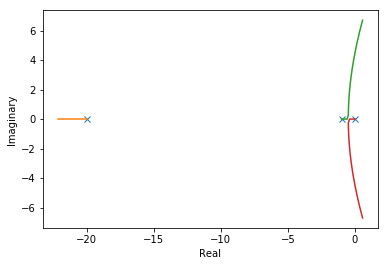
\includegraphics[width=0.7\linewidth]{Assignments/A1/ipython_files/qt_img486735758753796}
	\caption{Root Locus created using matplotlib and python control library}
	\label{fig:qtimg486735758753796}
\end{figure}
\begin{pythonscript}
	Kv = sympy.limit(s*Gs, s, 0)
	print('The velocity error Kv is:')
	print(Kv)
	mag, phase, omega = bode(sys)
	real, imag, freq = nyquist(sys,labelFreq=10)
\end{pythonscript}

\begin{figure}
	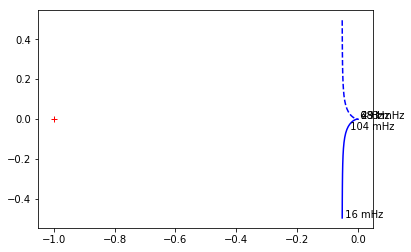
\includegraphics[width=0.7\linewidth]{Assignments/A1/ipython_files/qt_img494204706881540}
	\caption{Bode Plot}
\end{figure}

\begin{figure}
	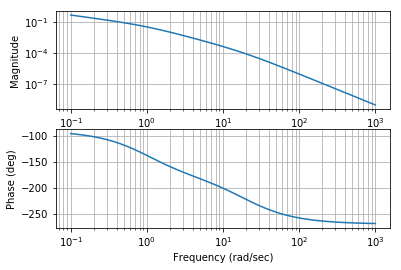
\includegraphics[width=0.7\linewidth]{Assignments/A1/ipython_files/qt_img492813137477636}
	\caption{Nyquist Plot}
\end{figure}

\section{Assignment 1 Reduced}
\subimport*{Assignments/A1/}{A1Reduced.tex}
\subimport*{Assignments/A2/}{ELEC460A2Content.tex}

\section{Assignment 3}
\subimport*{Assignments/A3/}{ELEC460A3Work.tex}
\section{Assignment 4}
\subimport*{Assignments/A4/}{ELEC460A4.tex}

\section{Assignment 5}
\subimport*{Assignments/A5/}{ELEC460A5.tex}

\section{Assignment 6}
\subimport*{Assignments/A6/}{elec460A6.tex}

\section{Assignment 7}
\subimport*{Assignments/A7/}{ELEC460A7PrintHandIn.tex}

\section{Assignment 8}
\subimport*{Assignments/A8/}{ELEC460A8HandIn.tex}

\section{Assignment 9}
\subimport*{Assignments/A9/}{ELEC460A9.tex}
\part{Back Matter}

\begin{proof}[This is a proof]
	Lwarp can solve my problems of creating good quality latex notes in html.
\end{proof}
\section*{List of Terms Used}
\gls{Actuator} \gls{LTI} \gls{MIMO} \gls{SISO} \gls{bodeDia} \gls{closedLoop} \gls{conSys} \gls{controlGain} \gls{cornFreq} \gls{critDamp} 
% Do not put a foot note at the front page again, a big mistake
%Some of the material include may be reused from previous courses \footnote{Note that I completed 3A before 3B}.


\chapter*{References}\label{references}
\addcontentsline{toc}{chapter}{References}

%\hypertarget{refs}{}
%\hypertarget{ref-book:129711}{}
%{[}1{]} Ogata, \emph{Discrete-time control systems}. {[}Online{]}.
%Available:
%\url{http://gen.lib.rus.ec/book/index.php?md5=18291B9E47990BD700872FE29FB417B9}
%
%\hypertarget{ref-textbook:niseSolution}{}
%{[}2{]} N. S. Nise, \emph{Control systems engineering - instructor
%	solutions manual}, 6th ed. Wiley, 2010 {[}Online{]}. Available:
%\url{http://gen.lib.rus.ec/book/index.php?md5=27a8107743faac0058228c0056a291fd}
%
%\hypertarget{ref-textbook:nise}{}
%{[}3{]} N. S. Nise, \emph{Control systems engineering}, 7th ed. Wiley,
%2015 {[}Online{]}. Available:
%\url{http://gen.lib.rus.ec/book/index.php?md5=d89ffd2789223fd1b3d1811615d1b3ba}
%
%\hypertarget{ref-book:DCSphil}{}
%{[}4{]} H. T. P. Chakrabortty Aranya; Nagle, \emph{``Digital control
%	system analysis and design: Global edition''}, 4th edition. Pearson
%Education Limited, 2015 {[}Online{]}. Available:
%\url{http://gen.lib.rus.ec/book/index.php?md5=9f61bcd95c74c37b4e0223ed7ef60ba9}
%
%\hypertarget{ref-book:209199}{}
%{[}5{]} B. Jähne, \emph{Digital control systems: Design, identification
%	and implementation}..
%
%\hypertarget{ref-textbook:ogataSolution}{}
%{[}6{]} K. Ogata, \emph{Solution manual for modern control engineering},
%5th ed. Prentice Hall, 2010 {[}Online{]}. Available:
%\url{http://gen.lib.rus.ec/book/index.php?md5=9b555958bb6c026c7c3387f13688f75e}
%
%\hypertarget{ref-textbook:ogata}{}
%{[}7{]} K. Ogata, \emph{Modern control engineering}, 5th ed. Prentice
%Hall, 2010 {[}Online{]}. Available:
%\url{http://gen.lib.rus.ec/book/index.php?md5=db54fc25ee52e896aa3a6c01592d1a79}
%
%\hypertarget{ref-textbook:dorf}{}
%{[}8{]} R. H. B. Richard C. Dorf, \emph{Modern control systems 12th
%	edition}, 12th ed. Prentice Hall, 2011 {[}Online{]}. Available:
%\url{http://gen.lib.rus.ec/book/index.php?md5=E61353006A43C7B8823A8F3012E9267D}
%
%\hypertarget{ref-textbook:dorfSolution}{}
%{[}9{]} R. H. B. Richard C. Dorf, \emph{Instructor's solutions manual
%	for modern control systems, 12th edition}, 12th ed. Prentice Hall, 2011
%{[}Online{]}. Available:
%\url{http://gen.lib.rus.ec/book/index.php?md5=814F498D384A3FC0B40F96FE5E213216}
%
%\hypertarget{ref-textbook:kuo}{}
%{[}10{]} B. C. K. Farid Golnaraghi, \emph{Automatic control systems 9th
%	edition}, 9th ed. Wiley, 2009 {[}Online{]}. Available:
%\url{http://gen.lib.rus.ec/book/index.php?md5=3A772763652D32CD43EAAB2D211BBCBA}
%
%\hypertarget{ref-textbook:kuoSolutions}{}
%{[}11{]} B. C. K. Farid Golnaraghi, \emph{Automatic control systems, 9th
%	edition - solutions manual}, 9th ed. Wiley, 2009 {[}Online{]}.
%Available:
%\url{http://gen.lib.rus.ec/book/index.php?md5=5E86FF471500C5E31E8A4655D62F0A89}
%
%\hypertarget{ref-essElec360:Online}{}
%{[}12{]} E. S. Society, ``Past exams elec 360 {[}online{]} available.''
%{[}Online{]}. Available: \url{http://ess.uvic.ca/exams/ELEC/}
%
%\hypertarget{ref-megaElec360:Online}{}
%{[}13{]} MEGA, ``Engineering student shared drive {[}online{]}
%available.'' {[}Online{]}. Available:
%\url{https://mega.nz/\#F!eJN1XLoI!cLb7ZYON1q53OeUFHShrJg!XcllnAhA}
%
%\hypertarget{ref-wiki:Cauchy}{}
%{[}14{]} Wikipedia, ``Cauchy's integral theorem --- wikipedia, the free
%encyclopedia.'' 2017 {[}Online{]}. Available:
%\url{https://en.wikipedia.org/w/index.php?title=Cauchy\%27s_integral_theorem\&oldid=778695526}
%
%\hypertarget{ref-MatlabCST}{}
%{[}15{]} MATLAB, ``MATLAB control systems toolbox.'' 2016 b.
%
%\hypertarget{ref-MatlabSMT}{}
%{[}16{]} MATLAB, ``MATLAB symbolic math toolbox.'' 2016 b.

% Works with lwarp 0.46, perhaps lwarp is the best approach to use now ahaha.
\nocite{*}
\printbibliography[heading=none]

%% generate plain text reference using pandoc conversion to html and copy and past

\addcontentsline{toc}{chapter}{Glossary}
\printglossaries

%\printindex
\end{document}